\documentclass{standalone}
\usepackage{amsmath}
\usepackage{amssymb}
\usepackage{tikz}
\usepackage{mathrsfs}
\usepackage{ifthen}

\newcommand{\perpp}{\perp\!\!\!\perp}
\DeclareMathOperator{\so}{\mathfrak{s}}
\DeclareMathOperator{\ra}{\mathfrak{r}}
\DeclareMathOperator{\supp}{supp}
\DeclareMathOperator{\id}{id}
\DeclareMathOperator{\dom}{dom}
\DeclareMathOperator{\ran}{ran}
\DeclareMathOperator{\Min}{Min}
\DeclareMathOperator{\cod}{cod}
\newcommand{\smallerthan}{<}
\newcommand{\greaterthan}{>}
\newcommand{\defeq}{:=}
\newcommand{\eqdef}{=:}

\newcommand{\cat}[1]{\textbf{#1}}
\DeclareMathOperator{\IG}{\mathscr{IG}}


\begin{document}
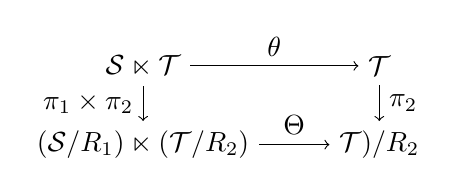
\begin{tikzpicture}
        \node (ST) at (0,0) {$\mathcal{S}\ltimes\mathcal{T}$};
        \node (T) at ([shift={+(3,0)}]ST) {$\mathcal{T}$};
        \node (SRTR) at ([shift={+(0,-1)}]ST) {$(\mathcal{S}/R_1)\ltimes(\mathcal{T}/R_2)$};
        \node (TR) at ([shift={+(0,-1)}]T) {$\mathcal{T})/R_2$};
        \draw[->] (ST)--(T) node[midway,above] {$\theta$};
        \draw[->] (ST)--(SRTR) node[midway,left] {$\pi_1\times\pi_2$};
        \draw[->] (T)--(TR) node[midway,right] {$\pi_2$};
        \draw[->] (SRTR)--(TR) node[midway,above] {$\Theta$};
    

\end{tikzpicture}\end{document}